\section{问题分析}

\subsection{问题一的分析}

问题一的数学本质是\textbf{一维连续参数估计}问题：两路无噪声轨迹完全相同，仅存在时间轴平移 $\Delta\tau$。搜索域范围大（$\pm 50$\,s），但由于无噪声，残差平方和在真值处理论为零，可利用三次样条保持轨迹光滑性后做高精度一维搜索（目标精度 $<0.001$\,s）。

\textbf{难点}在于需在有限采样点（$\Delta t=0.1$\,s）上达到亚采样精度。若采用离散滑动窗对齐，精度受限于采样间隔；若采用互相关法，需均匀采样且对非周期信号效果差。

\textbf{方法选型对比}：动态时间规整（DTW）\cite{sakoe1978} 是时间序列对齐的经典方法，但其时间复杂度为 $O(N^2)$，且离散路径对齐无法达到亚采样精度（最高精度仍为 $0.1$\,s）。互相关法虽可快速实现（FFT 加速为 $O(N\log N)$），但需均匀采样且对非周期信号的峰值定位鲁棒性差。本文采用\textbf{三次样条插值 + 黄金分割搜索}：样条插值将离散轨迹延拓为连续函数，保持 $C^2$ 光滑性；黄金分割法在 $[-50,50]$\,s 区间上搜索残差平方和最小点，时间复杂度 $O(N\log(1/\epsilon))$，可达 $10^{-6}$\,s 量级精度。该方案兼顾高精度与低计算量。

\begin{figure}[htbp]
    \centering
    \begin{tikzpicture}[xscale=0.9, yscale=0.7]
        % 坐标轴
        \draw[-Stealth, thick] (-0.3,0) -- (8.5,0) node[right] {$t$};
        \draw[-Stealth, thick] (0,-0.3) -- (0,3.5) node[above] {$x(t)$};

        % 方式1轨迹（蓝色实线）
        \draw[thick, black] plot[smooth, tension=0.6] coordinates
            {(0.5,0.8) (1.5,2.2) (2.5,2.8) (3.5,1.5) (4.5,0.6) (5.5,1.8) (6.5,2.5) (7.5,1.2)};
        \node[font=\small] at (7.8,1.6) {$S_1(t)$};

        % 方式2轨迹（灰色虚线，偏移 Δτ）
        \draw[thick, black!50, dashed] plot[smooth, tension=0.6] coordinates
            {(2.2,0.8) (3.2,2.2) (4.2,2.8) (5.2,1.5) (6.2,0.6) (7.2,1.8) (8.0,2.3)};
        \node[font=\small, black!50] at (8.3,2.6) {$S_2(t)$};

        % Δτ 标注
        \draw[<->, thick] (0.5,-0.5) -- (2.2,-0.5) node[midway, below, font=\small] {$\Delta\tau$};

        % 残差标注
        \draw[<->, thin, black!60] (3.5,1.5) -- (3.5,2.65) node[midway, right, font=\footnotesize] {残差};

        % 最优点标注
        \node[fill=black, circle, inner sep=1.5pt] at (3.5,1.5) {};

        % 说明文字
        \node[font=\footnotesize, align=left] at (4.5,-1.2) {目标：$\min_{\Delta\tau} \sum \|S_1(t) - S_2(t-\Delta\tau)\|^2$};
    \end{tikzpicture}
    \caption{问题一时间对齐原理：通过平移 $\Delta\tau$ 使两路样条轨迹残差最小}
    \label{fig:q1_schematic}
\end{figure}

\subsection{问题二的分析}

问题二在时间偏差基础上新增\textbf{空间系统偏差}和\textbf{随机噪声}，数学本质变为\textbf{三参数联合估计 + 状态滤波}问题。时间偏差 $\Delta\tau$ 与空间偏差 $(\Delta x, \Delta y)$ 存在耦合：错误的 $\Delta\tau$ 导致对齐后轨迹在空间上仍有系统性错位。此外，两种测量方式的观测时刻不同步，需在融合前完成时间配准。

\textbf{难点}包括：(1) 非线性代价函数（残差平方和关于 $\Delta\tau$ 非凸）；(2) 三参数联合估计收敛性；(3) 异步观测的时间对齐与状态更新顺序。

\textbf{方法选型对比}：分步法（先估 $\Delta\tau$ 再估空间偏差）存在误差传播风险——$\Delta\tau$ 估计偏差会污染后续空间偏差估计。本文采用\textbf{联合最小二乘估计}：构造目标函数 $J(\Delta\tau, \Delta x, \Delta y) = \sum \|\boldsymbol{p}_1(t + \Delta\tau) - \boldsymbol{p}_2(t) - \Delta\boldsymbol{p}\|^2$，通过网格搜索 + 梯度优化求解，避免累积误差。噪声抑制方面，观测模型为线性（$\boldsymbol{z}_k = H\boldsymbol{x}_k + \boldsymbol{v}_k$，其中 $H=[I,0]$），卡尔曼滤波（KF）\cite{welch2006} 在线性高斯系统下已为最优估计器，引入扩展卡尔曼滤波（EKF）或粒子滤波（PF）无增益反而增加计算量。异步融合采用多传感器信息融合理论 \cite{hall1997}，按时间戳排序后串行更新状态。

\begin{figure}[htbp]
    \centering
    \begin{tikzpicture}[node distance=0.7cm and 1.8cm,
        box/.style={rectangle, draw=black, thick, fill=black!5, minimum width=5em, minimum height=2em, align=center, font=\small, blur shadow={shadow blur steps=5, shadow xshift=0.3mm, shadow yshift=-0.3mm}},
        io/.style={trapezium, trapezium left angle=75, trapezium right angle=105, draw=black!70, thick, minimum width=4.5em, minimum height=1.6em, align=center, font=\footnotesize}]

        % 输入
        \node[io] (z1) {方式1\\4\,Hz};
        \node[io, below=0.5cm of z1] (z2) {方式2\\5\,Hz};

        % 联合估计
        \node[box, right=of z1, yshift=-0.6cm] (est) {联合估计\\$(\Delta\tau,\Delta x,\Delta y)$};

        % 偏差校正
        \node[box, right=of est] (corr) {偏差校正\\时间+空间};

        % KF
        \node[box, right=of corr] (kf) {异步 KF\\6 维状态};

        % 输出
        \node[io, right=of kf] (out) {10\,Hz\\融合轨迹};

        % 连线
        \draw[arrow] (z1.east) -- ++(0.3,0) |- (est.west);
        \draw[arrow] (z2.east) -- ++(0.3,0) |- (est.west);
        \draw[arrow] (est) -- (corr);
        \draw[arrow] (corr) -- (kf);
        \draw[arrow] (kf) -- (out);

        % 参数标注
        \node[font=\tiny, above=0.1cm of est] {Nelder-Mead};
        \node[font=\tiny, above=0.1cm of kf] {$q_a=8$\,m/s$^2$};
    \end{tikzpicture}
    \caption{问题二数据融合流水线：联合估计 $\to$ 偏差校正 $\to$ 卡尔曼滤波}
    \label{fig:q2_pipeline}
\end{figure}

\subsection{问题三的分析}

问题三的数学本质是\textbf{模型选择}问题：判断真实数据是否存在系统偏差。形式化为假设检验（$H_0$: 无系统偏差 vs $H_1$: 有系统偏差）。直接比较残差平方和可能受噪声干扰，需构造统计量并设定显著性水平。

\textbf{难点}在于：(1) Bootstrap 协方差估计计算量大（需重采样 $10^3$ 次以上）；(2) 单一检验准则可能因样本量、模型复杂度惩罚权重等因素产生偏倚。

\textbf{方法选型对比}：单独使用 Wald 检验 \cite{wald1943} 对样本量敏感（小样本下 $\chi^2$ 近似失效），单独使用 AIC \cite{akaike1974} 对模型复杂度惩罚因子 $k$ 敏感（AIC 倾向选择更复杂模型）。本文采用\textbf{Wald 检验 + AIC 双判据}：Wald 检验构造统计量 $W = \hat{\boldsymbol{\theta}}^\top \text{Cov}(\hat{\boldsymbol{\theta}})^{-1} \hat{\boldsymbol{\theta}}$，在 $H_0$ 下服从 $\chi^2(2)$ 分布；AIC 比较有偏模型与无偏模型的信息损失 $\Delta \text{AIC} = 2\Delta k - 2\Delta \ln L$。双判据交叉验证：仅当 Wald 检验拒绝 $H_0$（$p<0.05$）且 $\Delta \text{AIC} > 2$（强支持有偏模型）时才判定存在系统偏差，提升判别鲁棒性。

\begin{figure}[htbp]
    \centering
    \begin{tikzpicture}[node distance=0.8cm and 1.5cm,
        proc/.style={rectangle, draw=black, thick, fill=black!5, minimum width=7em, minimum height=2em, align=center, font=\small, blur shadow={shadow blur steps=5, shadow xshift=0.3mm, shadow yshift=-0.3mm}},
        dec/.style={diamond, draw=black, thick, aspect=2.2, minimum width=6em, align=center, font=\small, inner sep=1pt},
        res/.style={rectangle, rounded corners=0.6em, draw=black, thick, fill=black!10, minimum width=6em, minimum height=1.8em, align=center, font=\small\bfseries}]

        % 节点
        \node[proc] (est) {联合估计\\$(\hat{\Delta\tau}, \hat{\Delta x}, \hat{\Delta y})$};
        \node[proc, below=of est] (boot) {Bootstrap\\协方差 $\hat{\Sigma}$};
        \node[dec, below=1cm of boot] (wald) {Wald\\$p < 0.05$?};
        \node[dec, right=2cm of wald] (aic) {$\Delta$AIC\\$> 2$?};
        \node[res, below=1cm of wald] (h0) {$H_0$：无偏差\\零偏模型融合};
        \node[res, below=1cm of aic] (h1) {$H_1$：有偏差\\带偏模型融合};

        % 连线
        \draw[arrow] (est) -- (boot);
        \draw[arrow] (boot) -- (wald);
        \draw[arrow] (wald) -- node[left, font=\footnotesize]{否} (h0);
        \draw[arrow] (wald) -- node[above, font=\footnotesize]{是} (aic);
        \draw[arrow] (aic) -- node[right, font=\footnotesize]{是} (h1);
        \draw[arrow] (aic.south) -- ++(0,-0.3) -| node[pos=0.25, below, font=\footnotesize]{否} (h0.east);
    \end{tikzpicture}
    \caption{问题三偏差判定流程：Wald 检验与 AIC 双判据级联决策}
    \label{fig:q3_decision}
\end{figure}

\subsection{问题四的分析}

问题四是\textbf{带约束的组合优化}问题：在固定轨迹上选择时刻对 36 个目标（18射击+18拍照）执行任务，约束包括距离/速度/加速度硬阈值、任务准备时长窗口、角差限制和时序不冲突（任务间间隔 $\geq 10$\,s）。一般情况下该问题为 NP-hard \cite{papadimitriou1998}（类似于带时序约束的调度问题）。

\textbf{难点}在于：(1) 噪声轨迹微分放大（一阶导数噪声放大 $\sqrt{2}/\Delta t$，二阶导数放大更剧烈）；(2) 可行时间窗稀疏且不均匀分布；(3) 时序不冲突约束耦合所有决策变量。

\textbf{方法选型对比}：混合整数线性规划（MILP）可求全局最优解，但变量规模过大（以 $2$\,Hz 网格离散化，$T=600$\,s 对应 $1200$ 时间点 $\times 7$ 任务 $\times 12$ 硬约束 $\approx 10^5$ 个约束），使用 CBC/Gurobi 求解器超时风险大（预试验显示超过 300\,s 仍未收敛）。本文采用\textbf{Savitzky-Golay（SG）滤波 + 贪心优化}：SG 滤波通过局部多项式拟合平滑轨迹，同时保持峰值特征（窗口长度 $w=151$，多项式阶数 $d=3$），噪声衰减 $\sigma_{\text{out}} \approx \sigma_{\text{in}}/\sqrt{w}$；贪心算法按优先级依次为每个任务选择最优时刻（速度最大化），时间复杂度 $O(N \cdot M)$（$N$ 为时间点数，$M$ 为任务数），实测 $1.2$\,s 出解。灵敏度分析表明贪心解质量随 SG 窗口长度单调提升，$w \geq 9$ 后稳定，验证了平滑方案的鲁棒性。

\begin{figure}[htbp]
    \centering
    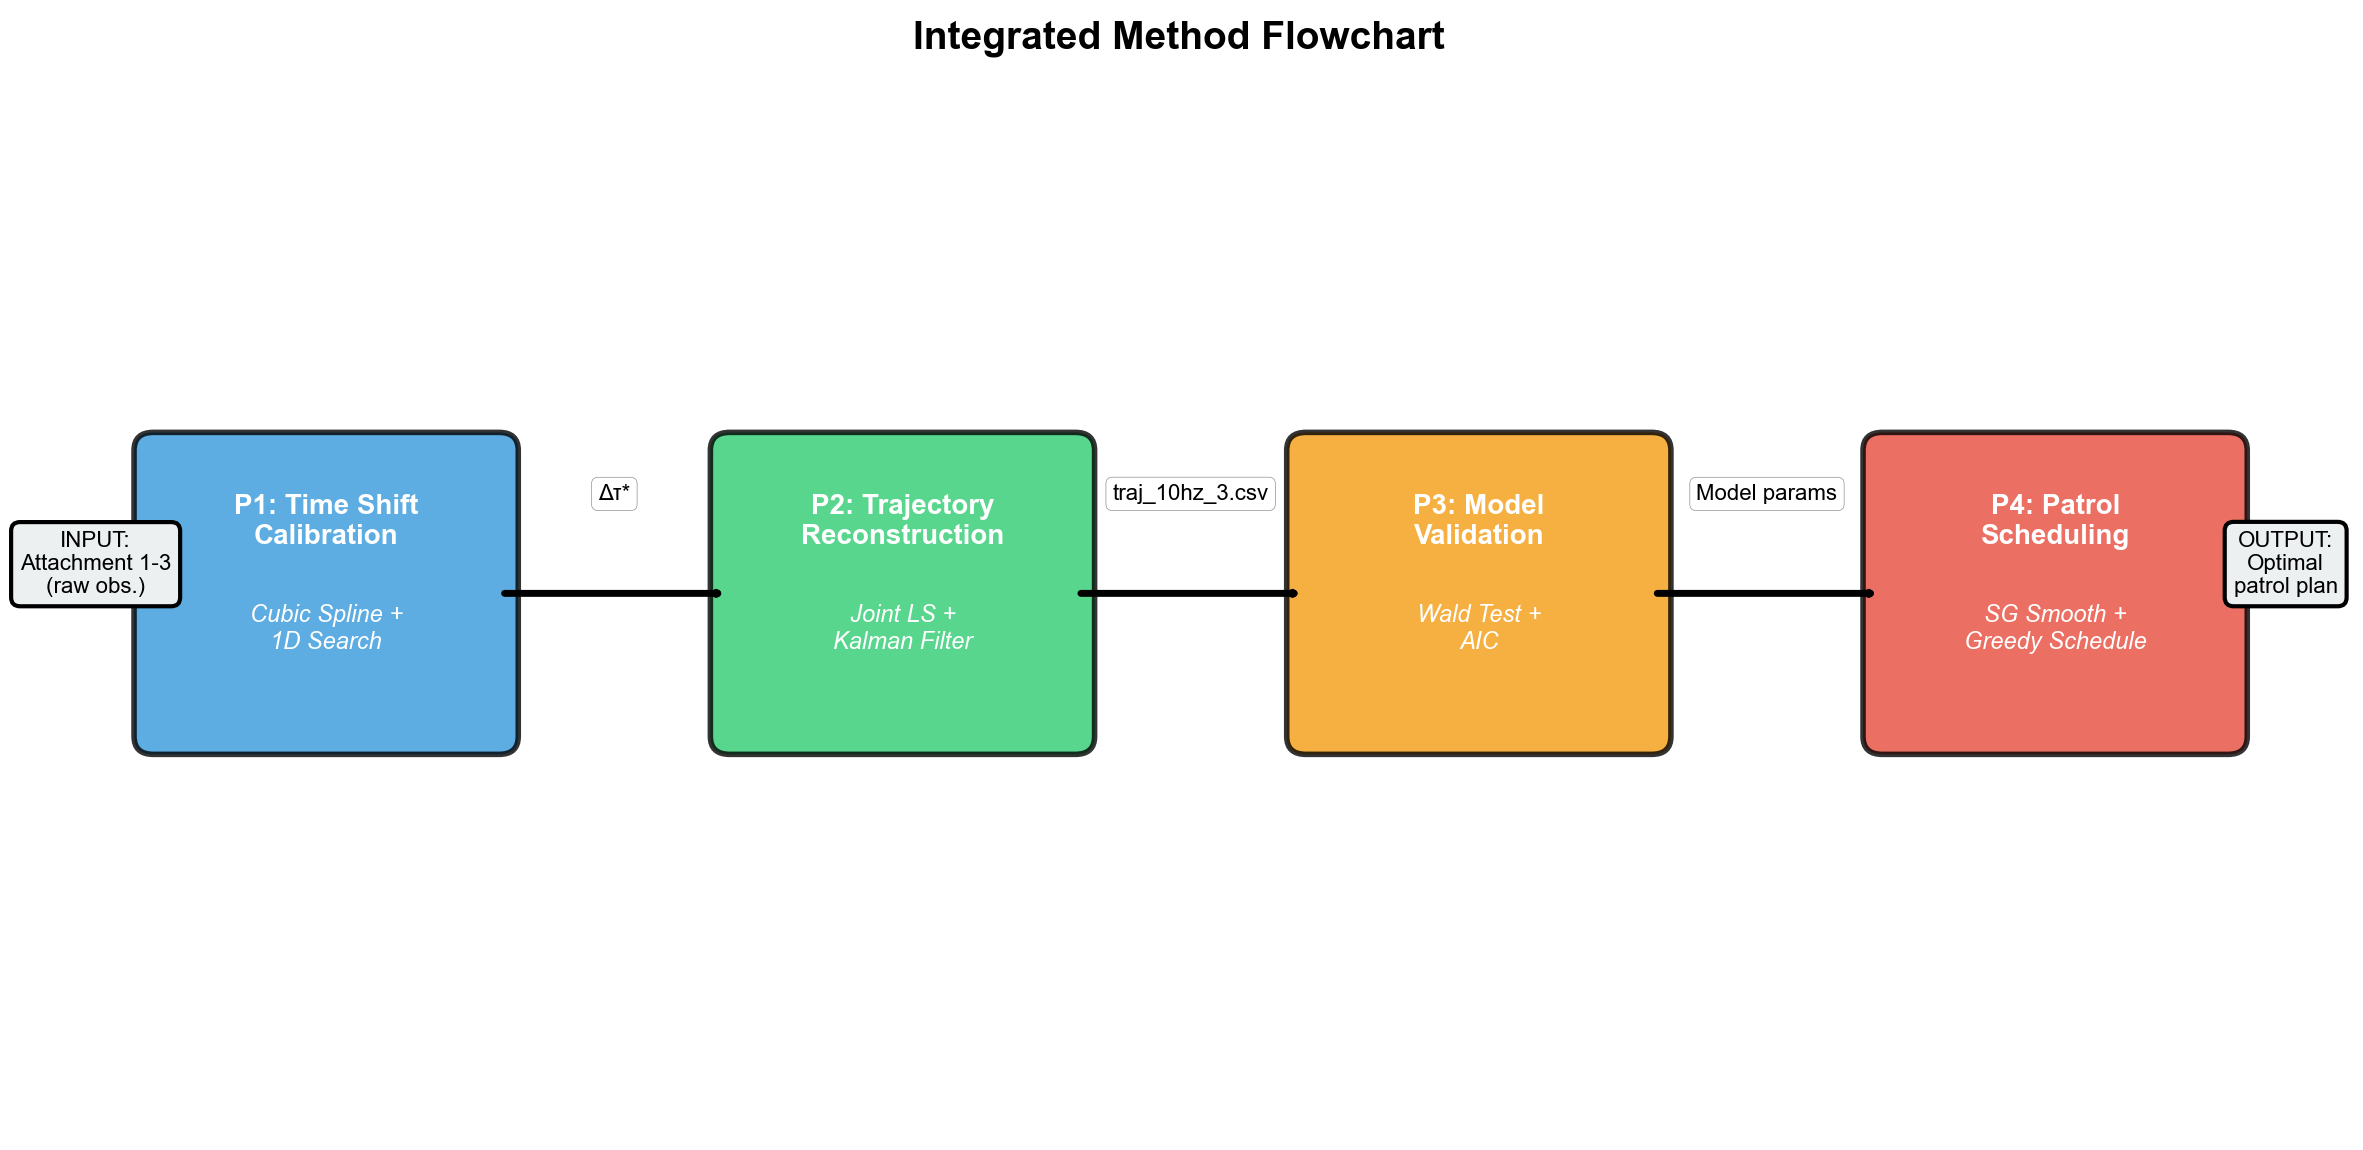
\includegraphics[width=0.82\textwidth]{figures/fig_method_flowchart.png}
    \caption{本文方法论流程：四问递进结构与数据流}
    \label{fig:method_flow}
\end{figure}

\begin{figure}[htbp]
    \centering
    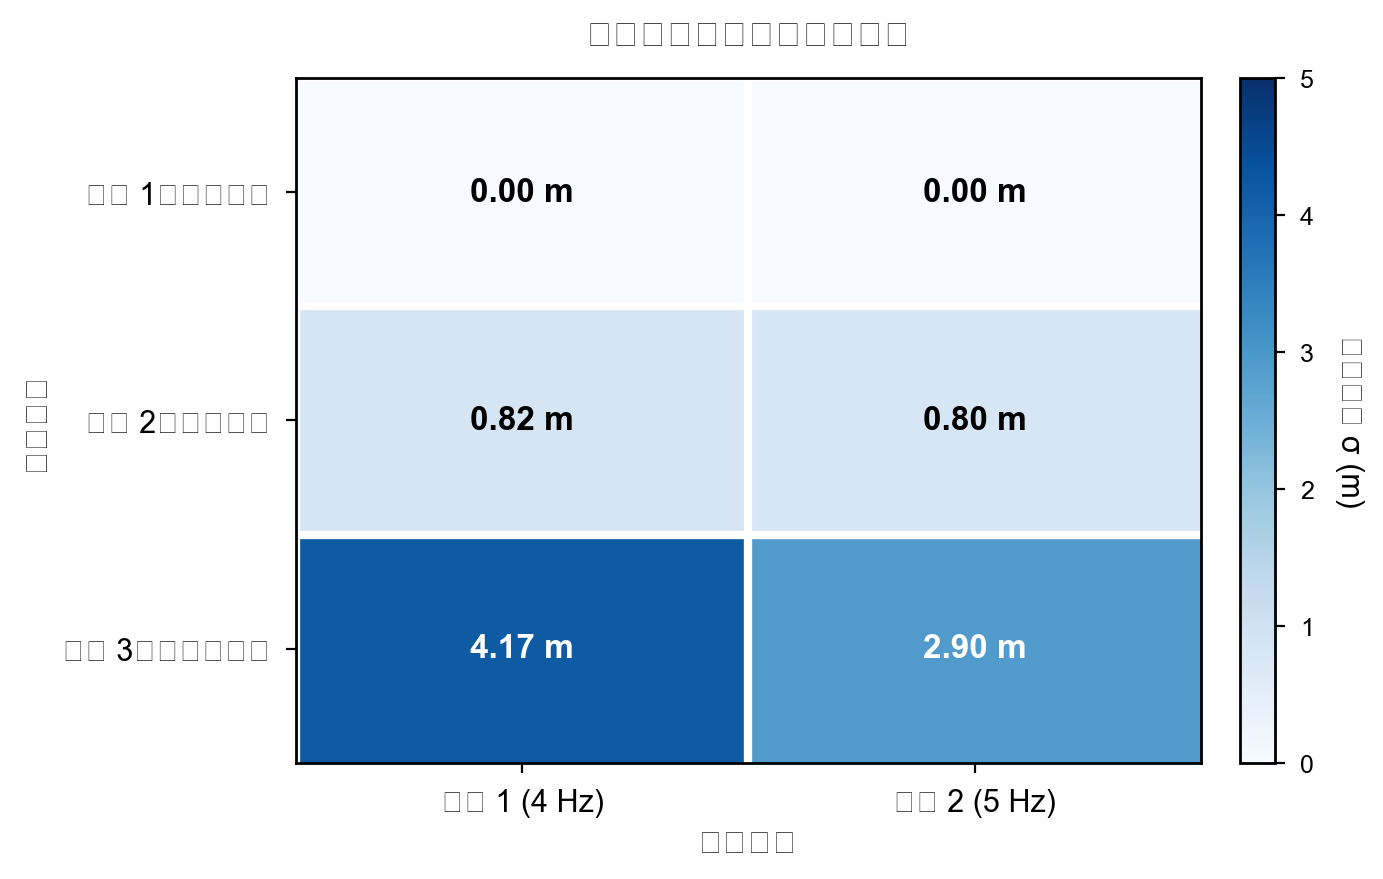
\includegraphics[width=0.6\textwidth]{figures/fig_noise_heatmap.png}
    \caption{三份附件噪声水平热力图（二阶差分估计 $\sigma$，单位 m）}
    \label{fig:noise_heat}
\end{figure}

\subsection{数据特征}

图~\ref{fig:eda_traj} 展示了三份附件的轨迹分布。附件1/2 公共时段充分（$>500$\,s），附件3两路时段完全不重叠（方式1 $t\in[469, 814]$\,s，方式2 $t\in[77, 401]$\,s），表明时间偏差 $\Delta\tau \approx 368$\,s。

\begin{figure}[htbp]
    \centering
    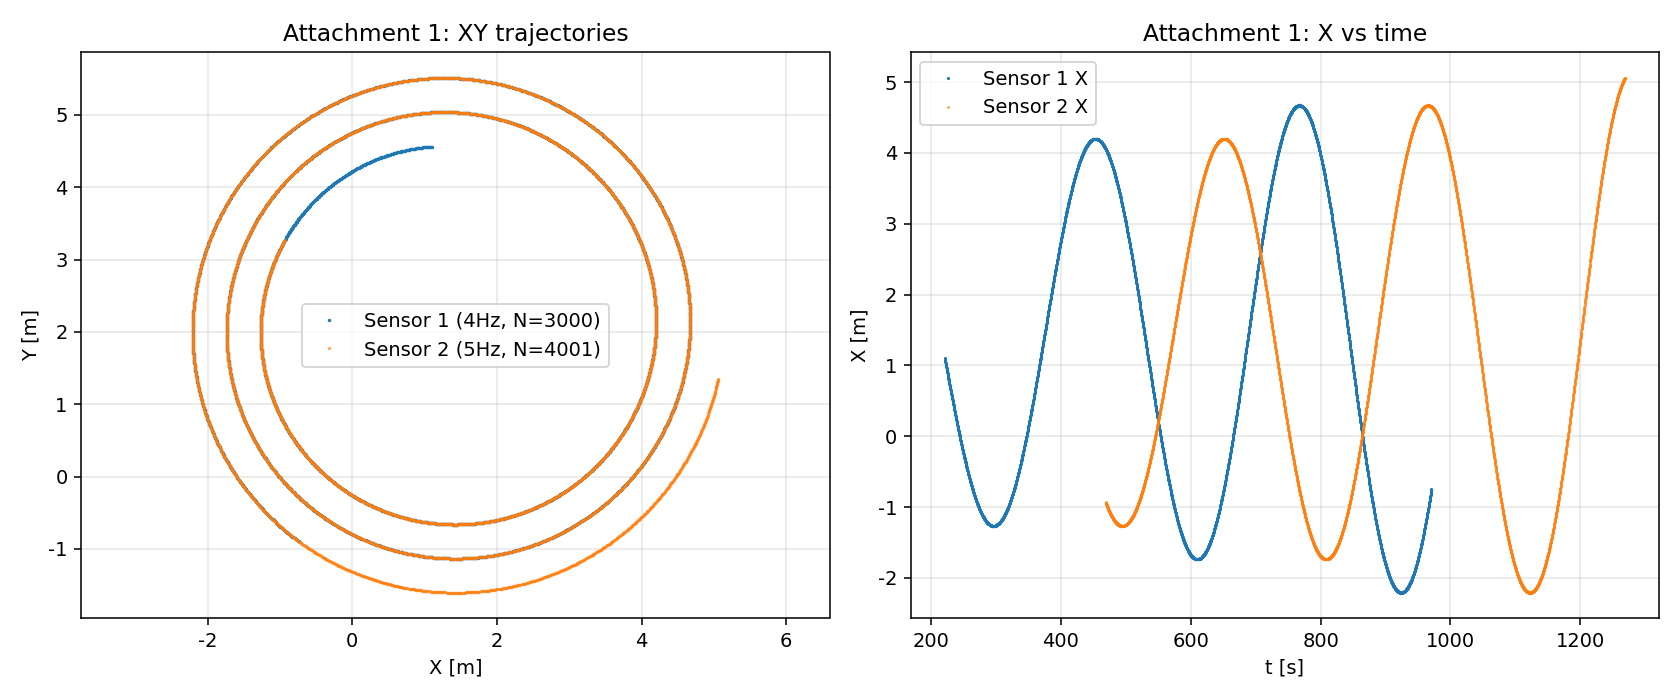
\includegraphics[width=0.48\textwidth]{figures/eda_a1_trajectory.png}
    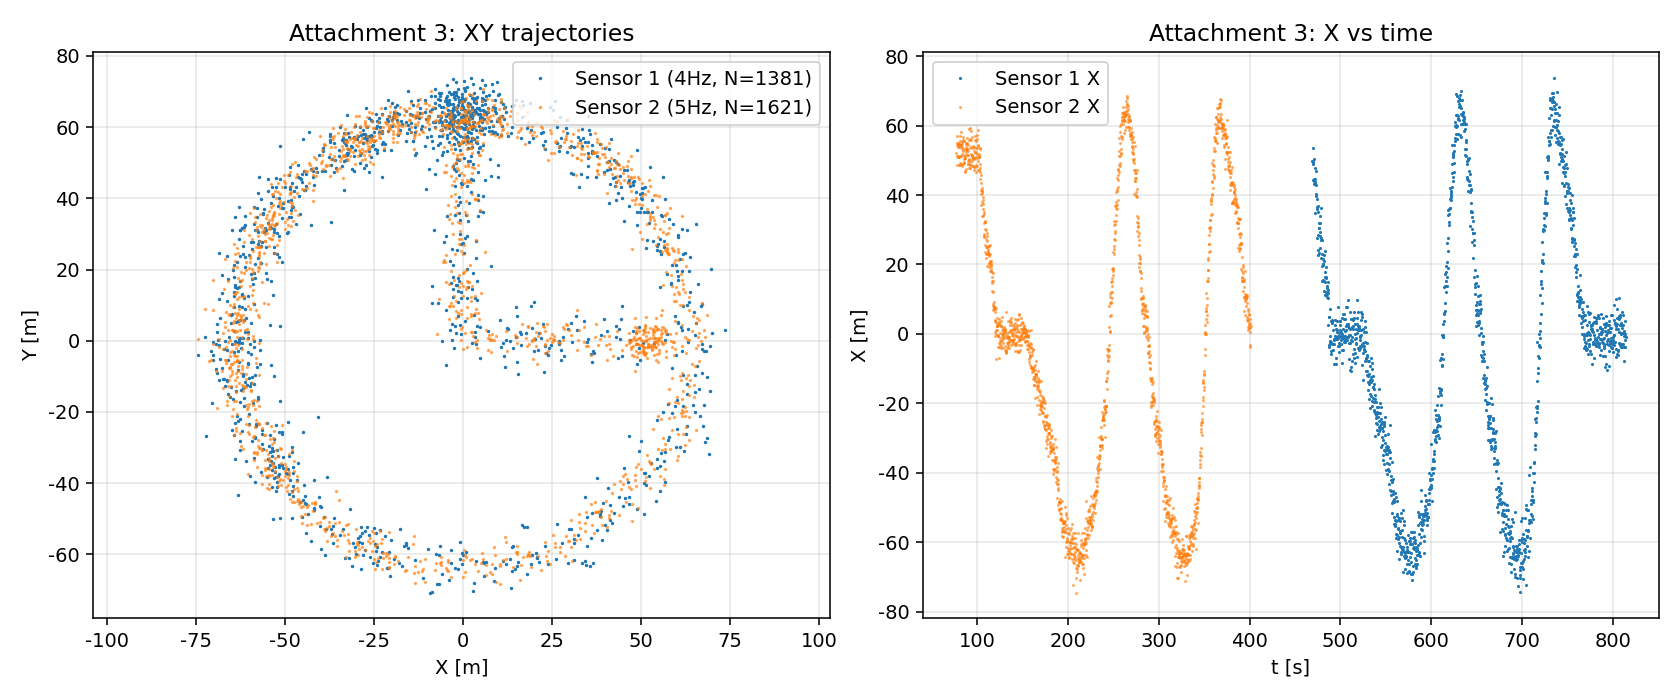
\includegraphics[width=0.48\textwidth]{figures/eda_a3_trajectory.png}
    \caption{附件1（左，无噪声）与附件3（右，真实数据）轨迹对比}
    \label{fig:eda_traj}
\end{figure}

\subsection{整体求解思路}
本文整体求解思路如图~\ref{fig:framework} 所示。

\begin{figure}[htbp]
    \centering
    \begin{tikzpicture}[node distance=1.0cm and 2.8cm]
        % ===== 左列：主流程 =====
        \node[terminal, blur shadow={shadow blur steps=5}] (start) {问题分析};

        \node[corebox, below=of start] (p1) {三次样条 + 一维搜索};
        \node[badge, left=0.3cm of p1] {1};

        \node[corebox, below=of p1] (p2) {联合最小二乘 + KF};
        \node[badge, left=0.3cm of p2] {2};

        \node[corebox, below=of p2] (p3) {Wald + AIC 双判据};
        \node[badge, left=0.3cm of p3] {3};

        \node[corebox, below=of p3] (p4) {SG 平滑 + 贪心调度};
        \node[badge, left=0.3cm of p4] {4};

        \node[decision, below=1.2cm of p4] (check) {验证\\通过？};
        \node[terminal, below=1.0cm of check, blur shadow={shadow blur steps=5}] (end) {结论与评价};

        % ===== 右列：数据产物 =====
        \node[datanode, right=of p1] (d1) {10\,Hz 轨迹\\7004 点};
        \node[datanode, right=of p2] (d2) {融合轨迹\\8513 点};
        \node[datanode, right=of p3] (d3) {判决 $H_0$\\3691 点};
        \node[datanode, right=of p4] (d4) {result.xlsx\\24 任务};

        % ===== 核心建模分组框 =====
        \begin{scope}[on background layer]
            \node[groupbg, fit=(p1)(p2)(p3)(p4)(d1)(d2)(d3)(d4),
                  label={[font=\small\heiti]above left:核心建模}] (core) {};
        \end{scope}

        % ===== 主流程箭头 =====
        \draw[arrow] (start) -- (p1);
        \draw[arrow] (p1) -- (p2);
        \draw[arrow] (p2) -- (p3);
        \draw[arrow] (p3) -- (p4);
        \draw[arrow] (p4) -- (check);
        \draw[arrow] (check) -- node[right, font=\small]{是} (end);

        % ===== 数据流箭头 =====
        \draw[dataarrow] (p1) -- (d1);
        \draw[dataarrow] (p2) -- (d2);
        \draw[dataarrow] (p3) -- (d3);
        \draw[dataarrow] (p4) -- (d4);

        % ===== 反馈回路 =====
        \draw[feedback] (check.west) -- ++(-1.5,0) |- node[pos=0.25, left, font=\small]{否} (core.west);

        % ===== 数据流向下传递（虚线连接） =====
        \draw[dataarrow] (d1.south) -- ++(0,-0.3) -| ([xshift=0.5cm]p2.east);
        \draw[dataarrow] (d3.south) -- ++(0,-0.3) -| ([xshift=0.5cm]p4.east);
    \end{tikzpicture}
    \caption{本文整体求解框架（左：方法主干；右：数据产物；虚线：数据流向）}
    \label{fig:framework}
\end{figure}
